% !TeX encoding = UTF-8
% !TeX spellcheck = en_US
% !TeX root = ledgersmb-book.tex

\part{Business processes}
\label{part-business-processes}

\chapter{Overview}
\label{cha-business-processes-overview}

This part of the document describes how LedgerSMB handles specific business processes.  For example, Order Entry, Shipping, etc.

Some of these processes may not apply to your specific use of the software and
can be ignored.

\chapter{Customers and vendors}
\label{cha-business-processes-customers}

\section{Introduction}
\label{sec-business-processes-customers-intro}

This section describes
how LedgerSMB implements \glspl{customer} and \glspl{vendor}.

When creating a customer or vendor in LedgerSMB, you have to first create a \gls{contact}. 
This contact can be created as either a \gls{company} or person.
However, this contact
can't itself be used directly as a \gls{vendor} or \gls{customer}. Instead, you have to create a ``\gls{credit account}''
which is linked to the contact. A ``\gls{credit account}'' can have the role of vendor, customer or both.

LedgerSMB works equally well using a person as a vendor, customer, or both.

A contact can have multiple \gls{customer} and/or \gls{vendor} type accounts. Each account has its
own language settings, shipping address, contact data and payment conditions.
Basically, you will create multiple accounts when you have to record different data
for any of the items listed above.

Note that at least as of LedgerSMB 1.9, a contact can only be linked to one bank account.  This means that if your contact as a vendor has separate bank accounts from your contact as a \gls{customer}, you will need to set them up as different contacts.

The contact entity itself is used - albeit not as customer or vendor - in the context of
credit risk management (See \charef{cha-credit-risk-management}).

\section{Creating customers and vendors}
\label{sec-business-processes-creating-customers-and-vendors}

The typical procedure to create customers and vendors works exactly alike:

\begin{enumerate}
\item Create the \gls{contact} as a company
\item Create \glspl{credit account}
\item Attach addresses, contact info and notes to the accounts
\end{enumerate}

\subsection{Creating a Company}
\label{subsec-business-processes-customer-creating-company}

To create a company navigate to Main Menu \ma Contacts \ma Add Contact \ma Company Tab.

The company tab has the following fields:

\begin{description}[style=nextline]
\item [Control code] Code to uniquely identify this entity.  This is usually generated by clicking on \texttt{Generate Control Code} button.  It is also generated automatically when clicking the \texttt{Save} button.
\item [Class] The type of entity; \gls{vendor}, \gls{customer}, etc. Required, but defaults to a known value so it needs to be checked.
\item [Name] Legal name of the company. Required.
\item [Country] Country of incorporation. Required, but defaults to a known value so it needs to be checked.
\item [Tax number/SSN] Tax (VAT/Sales tax) number of the company.
\item [Sales Tax ID] The sales tax reporting number.
\item [License Number] The company operating license number.
\end{description}

The \texttt{Generate Control Code} button generates a new control code upon
user request when the user is entering a company which isn't yet known
in the system in any other role.

The \texttt{Retrieve} button is discussed in \secref{sec-business-processes-customers-to-vendors}.

The \texttt{Save} button creates the account.

\subsection{Creating a customer account}
\label{subsec-business-processes-customers-creating-account}

When a contact of class ``Customer'' or ``Vendor'' has been created,
accounts of that type can be added. The account entry screen lists the
following fields\footnote{To simplify the interface if they're unused, some fields
are not shown in case their selection lists are empty}:

\begin{description}[style=nextline]
\item [Class] Either a \gls{customer} or \gls{vendor} 
\item [Number] Number to identify this account among all other accounts in the company; when left empty, the system will generate one when you click ``Save New''
\item [Description] Textual representation of the account, usually a name
\item [Pay To] @@@TODO
\item [Starting Date] Date from which the account is valid
\item [End date] Date until which the account is valid, or empty if there's no known end date
\item [Threshold] Minimum amount for invoices to be sent out
\item [Credit limit] Maximum amount of open invoices and orders allowed for the account, see \charef{cha-credit-risk-management}
\item [Payment Terms] Number of days within which invoices have to be paid
\item [Discount (conditions)] Percentage discount the account is entitled to when payment is within the given number of days
\item [Discount (account)] Account used to post discounts as calculated based on discount conditions
\item [AR] For customers, the Receivables G/L Account used to post created sales invoices on
\item [AP] For vendors the Payables G/L Account used as default to post received purchase order invoices on
\item [Payment] Which bank account to use when receiving or paying funds
\item [Currency] The default currency to be used with the \gls{customer} or vendor
\item [Language] The language parameter is used to select templates for communication with the customer
\item [Taxes] The applicable tax form for this vendor; tax forms are discussed in more detail in \secref{subsec-business-processes-accounting-reporting-tax-with-taxforms}
\charef{cha-taxes}
\end{description}

\subsection{Creating a vendor account}
\label{subsec-business-processes-vendors-creating-account}

Generally the only difference between creating a \gls{customer} account and a \gls{vendor} account is the Class and the use of AP or AR G/L accounts. See \secref{subsec-business-processes-customers-creating-account} for setting up a customer account.

\section{Multiple customers within one company}
\label{sec-business-processes-customer-multiple-per-company}

\section{Creating vendors from customers}
\label{sec-business-processes-customers-to-vendors}

% \section{}

\section{Maintaining contact information}
\label{sec-business-processes-customers-contact-information}


\chapter{Quotations from Vendors and for Customers}
\label{cha-business-processes-quotations}

\section{Creating Quotations and RFQs}
\label{sec-business-processes-quotations-creation}

% ### Proze with explanation missing

\begin{figure}[h]
\centering
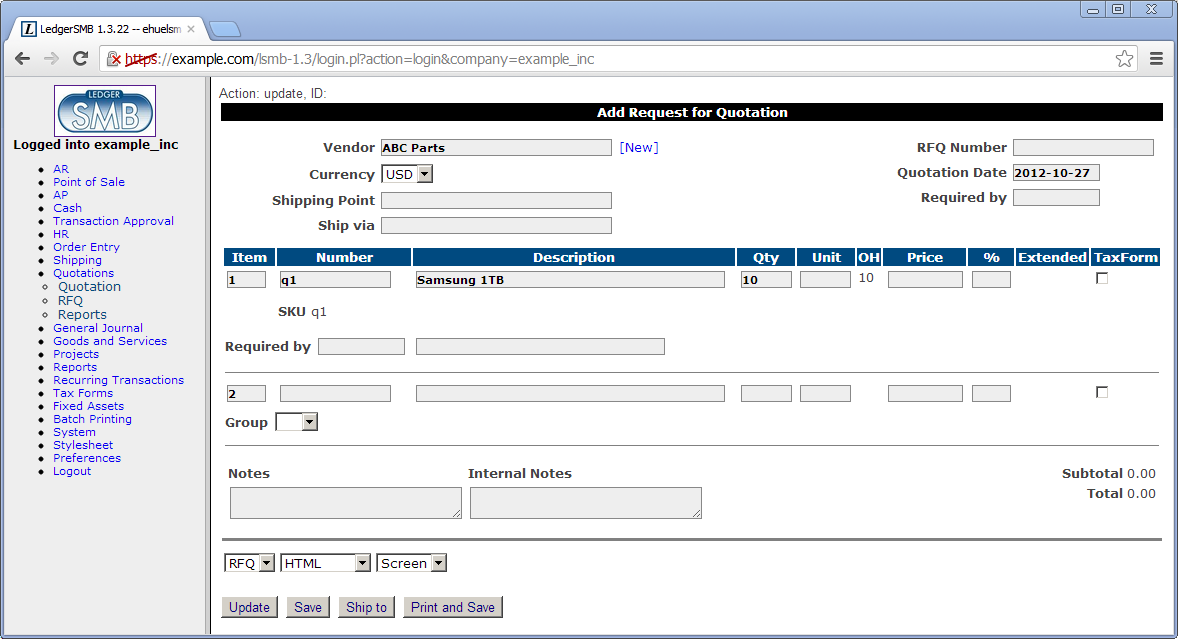
\includegraphics[width=\linewidth]{rfq-entry-screen.png}
\caption{RFQ entry screen}
\label{fig:rfq-entry-screen}
\end{figure}

\begin{quote}
\textbf{Remark} Note that the \gls{rfq} entry screen contains prices; this is misleading
at least: the printed output to be sent to the vendor does not. The fact that this screen
allows entry of prices could be considered a bug.
\end{quote}

The listing below describes the meaning of the per \gls{rfq} fields presented in the screen.

\begin{description}[style=nextline]
\item [Vendor (Customer)] Name of the company the quotation is requested from (issued to)
\item [Currency] Currency for the intended transaction
\item [Shipping point] Address to ship to ??? % ### TODO check with Chris
\item [Ship via] Shipping method ???  % ### TODO check with Chris
\item [RFQ number] The number of the document (automatically generated when left empty)
\item [Quotation date] Date the document is issued
\item [Required by] Date of the intended delivery of the goods and services requested ??? % ###
\item [Notes] Notes to be included on the printed RFQ document sent to the vendor
\item [Internal notes] Notes to be kept internal to the company - not disclosed through the RFQ document
\end{description}

The following per item fields are listed.

\begin{description}[style=nextline]
\item [Item] Order number of the item
\item [Number] Part number of the item to be ordered
\item [Description] Description or name of the item to be ordered
\item [Qty] The number of items to be ordered
\item [Unit] The unit in which the quantity is measured; e.g. 'each' or '6pack'
\item [OH] Number of items currently on hand (i.e. in stock)
\item [Price] Item price
\item [\%] Discount percentage rate
\item [Extended] Item price after discount
\item [TaxForm] % ### ???
\item [SKU] Stocking unit - code used to track stock
\item [Required by] Required date of delivery; can be used to specify a different date
   than the date in the header
\item [Remarks] Item specific remarks
\item [Group] (Not shown in the screen shot) Part group for the item
\end{description}

Note that the quotation entry screen offers a number of extra buttons after the data has
been saved.

\section{Expediting quotations}
\label{sec-business-processes-quotations-sending}

\subsection{Printing}
\label{subsec-business-processes-quotiontions-sending-print}

\subsection{Sending by e-mail}
\label{subsec-business-processes-quotations-sending-email}

\section{Attaching files to quotations}
\label{sec-business-processes-quotations-file-attachments}


\chapter{Sales and vendor orders}
\label{cha-business-processes-orders}

In this chapter the options for creating orders will be discussed.
After successful order creation, there are two possible next steps.
The first applies to cases where actual goods have to be handled
and goes through shipping and receiving as discussed in
\charef{cha-business-processes-inventory}. The other skips handling of goods
and directly proceeds to invoicing in \charef{cha-business-processes-invoicing}.

\section{Creating new orders}
\label{sec-business-processes-orders-creation}

\section{Creating orders from quotations}
\label{sec-business-processes-orders-creation-from-quotations}

\section{Creating orders from projects}
\label{sec-business-processes-orders-creation-from-projects}

@@@ What about from time sheets??

\section{Creating purchase orders from sales orders}
\label{sec-business-processes-orders-purchase-from-sales}

\section{Combining orders}
\label{sec-business-processes-orders-combining}


\section{Recurring orders}
\label{sec-business-processes-orders-recurring}

% @@@ ### Not getting these to work in the test system. Need to check with Chris.

\section{Incomplete orders}
\label{sec-business-processes-orders-incomplete}

Orders fully shipped and invoiced are automatically closed. However, this isn't always an option.

In case an order ends up being partially shipped and parties agree not to ship the remaining
items in the order, the order stays open and incomplete. In situations like these, the order
needs to be marked ``Closed'' in the order entry screen. A note stating why the order was manually
closed can be put in the ``Internal Notes'' input box. Clicking the ``Save'' button stores the
changes in the application database.


\chapter{Inventory management}
\label{cha-business-processes-inventory}

\section{Shipping}
\label{sec-business-processes-inventory-shipping}

\subsection{Pick lists}
\label{subsec-business-processes-inventory-shipping-picklist}

@@ \textbf{Order picking} is the work(flow), not the picklist!

\subsection{Packing list}
\label{subsec-business-processes-inventory-shipping-packlist}

@@ \textbf{Order packing} is the work(flow), not the packlist!

\section{Receiving}
\label{sec-business-processes-inventory-receiving}

@@@TODO the role of shipping points in receipts??

Reception of goods into inventory assumes having at least one
saved and incomplete purchase order such as shown in
\figref{fig:purchase-order-screen} stored in the system.

\begin{figure}[h]
\centering
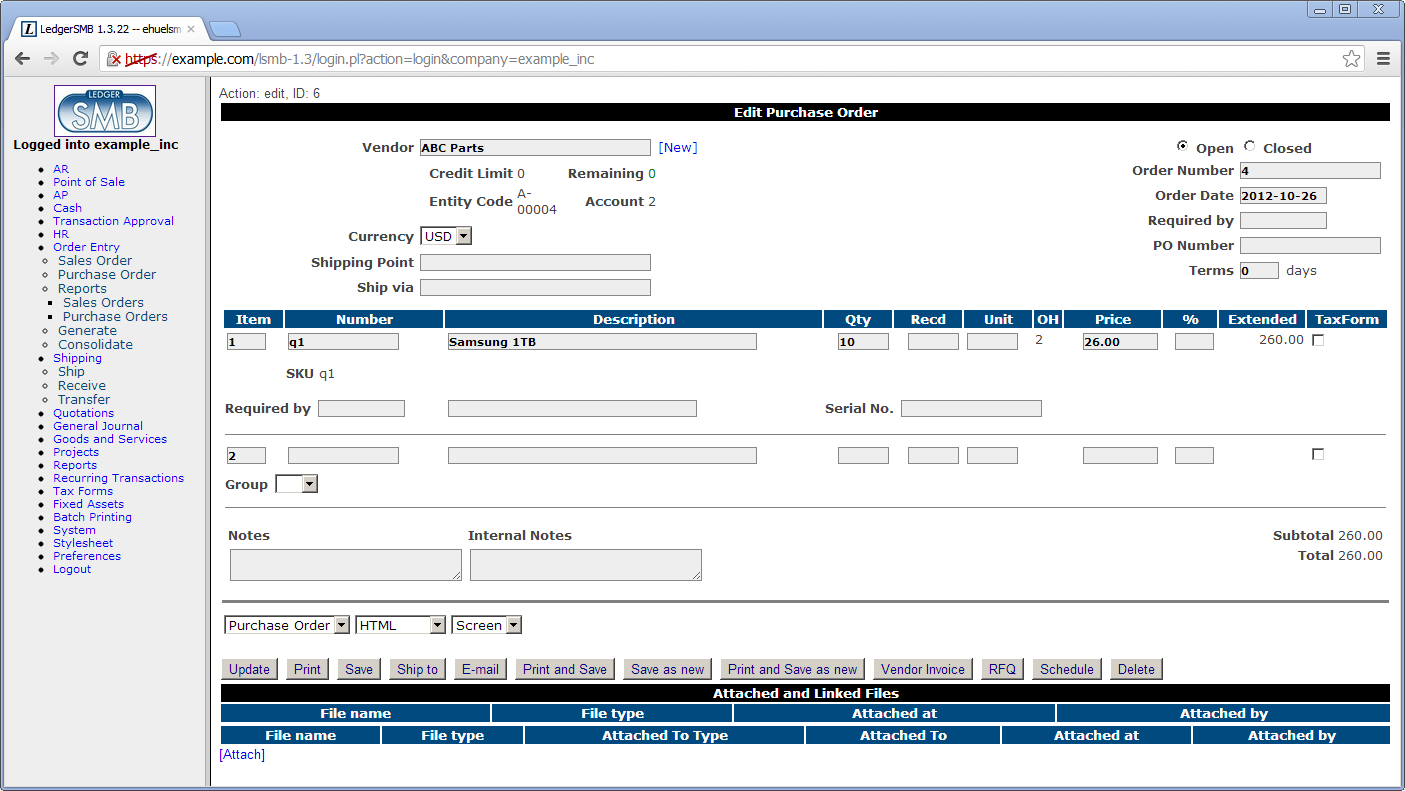
\includegraphics[width=\linewidth]{purchase-order-screen.png}
\caption{Saved purchase order}
\label{fig:purchase-order-screen}
\end{figure}

The reception process starts by going through the menu to the
``Receive'' order lookup screen (\menupath{Shipping \ma Receive}).
This will show the order search screen which will help finding
any orders which have items available for reception, see \figref{fig:shipping-receive-search-screen}.


\begin{figure}[h]
\centering
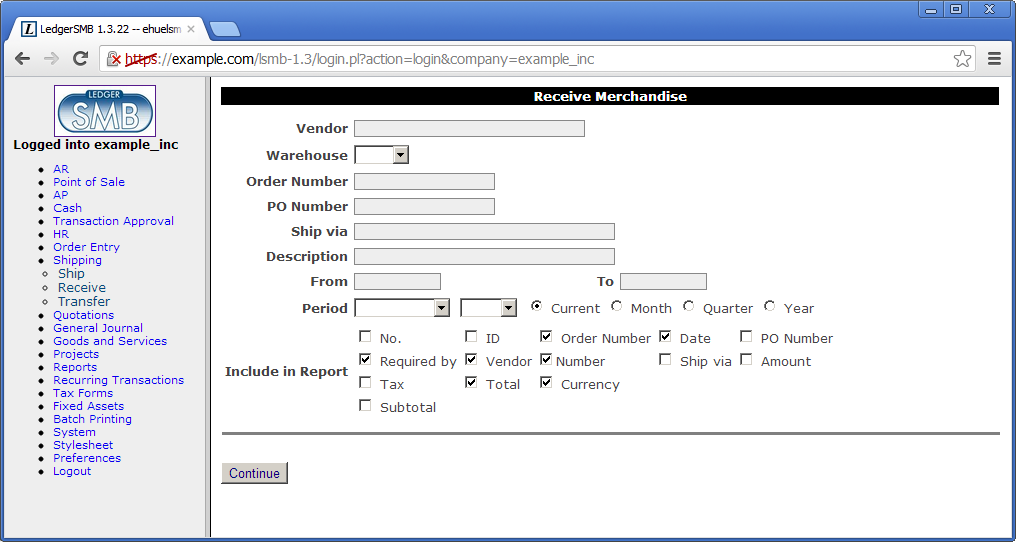
\includegraphics[width=\linewidth]{shipping-receive-search-screen.png}
\caption{Search screen for purchase order item receipts}
\label{fig:shipping-receive-search-screen}
\end{figure}

After filling order selection criteria and hitting the ``Continue'' button (or doing so
immediately to see all orders with outstanding items in the system), the system will return
a listing of orders with matching the selection criteria as in \figref{fig:shipping-receive-search-result-screen}.

\begin{figure}[h]
\centering
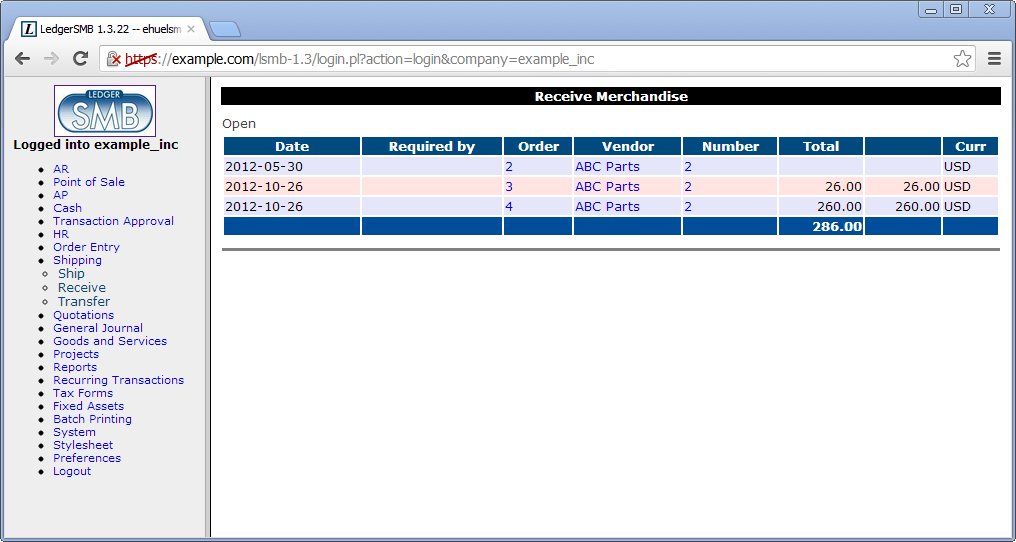
\includegraphics[width=\linewidth]{shipping-receive-search-result-screen.png}
\caption{Search results screen for purchase order item receipts}
\label{fig:shipping-receive-search-result-screen}
\end{figure}

Upon selection of one of the orders by clicking the order number the next screen is loaded
as shown in \figref{fig:shipping-receive-screen}. In this screen you can enter the amounts
received in the current lot. The entered data is to be confirmed with the ``Done'' button.
After confirmation of the receipt screen, items will be added to inventory.

\begin{figure}[h]
\centering
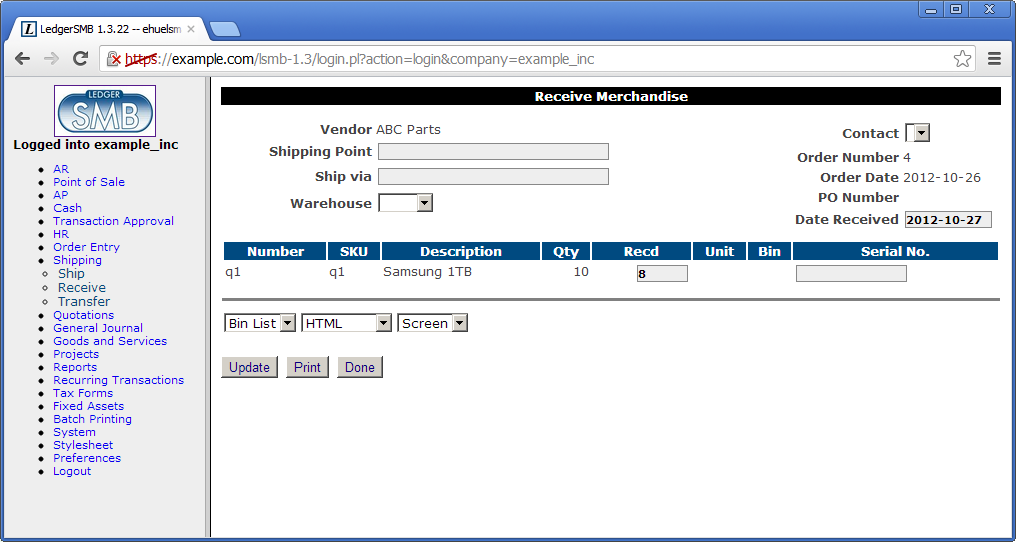
\includegraphics[width=\linewidth]{shipping-receive-screen.png}
\caption{Purchase order receipt screen}
\label{fig:shipping-receive-screen}
\end{figure}

LedgerSMB supports warehouse management on the Receipt screen by offering the ability to
print a ``Bin List''. This list contains the bin (storage) locations configured for each part.


\section{Partial shipments or receipts}
\label{sec-business-processes-inventory-shipping-partial}

Both shipping and receiving support partial shipments and per-lot invoicing. If the vendor
ships multiple lots to a single order (and charges a single invoice), you can simply call
up the order and enter items into inventory on the same order. The outstanding items
are automatically decremented by the amounts entered before.

To create an invoice for a received lot simply follow the process as detailed in
\secref{sec-business-processes-invoicing-from-orders}. If the lot is a partial shipment, the invoice will be
for the current receipt by default.

\section{Handling returns}
\label{sec-business-processes-inventory-shipping-returns}


\section{Transferring between warehouses}
\label{sec-business-processes-inventory-warehouse-transfers}

\section{Inventory reporting}
\label{sec-business-processes-inventory-reporting}

\subsection{Inventory status report}
\label{subsec-business-processes-inventory-reporting-status}

\subsection{Inventory activity report}
\label{subsec-business-processes-inventory-reporting-activity}




\chapter{Sales and vendor invoice handling}
\label{cha-business-processes-invoicing}

Invoices can come from multiple sources. When the quotation and order
management functionalities in LedgerSMB aren't used, they will usually
be entered manually. This work flow is covered in Section
\ref{sec-business-processes-invoicing-manual-entry}.
When order management \emph{is} being used they mostly originate from orders
which is covered in Section \ref{sec-business-processes-invoicing-from-orders}.



\section{Creating invoices from orders}
\label{sec-business-processes-invoicing-from-orders}

% This section first because the previous chapter is about orders,
% which seems like a natural flow for the book




\section{Creating new invoices}
\label{sec-business-processes-invoicing-manual-entry}


%% this section is about Sales and Vendor Invoices

When a business decides not to use the order management as per the previous
chapter it may find itself in need to manually enter invoices. But even
if it does use order management, it may be necessary to enter an invoice
directly.

When creating a transaction to record that the company owes another
entity (a vendor invoice) or that it has outstanding receivables,
LedgerSMB offers two options:

\begin{enumerate}
\item Invoices
\item Transactions
\end{enumerate}

Transactions have very limited functionality: they allow a user to enter
a debt owed or owned into the AR and AP subsystems. They also require the
user to think how the other side of the transaction should be registered;
i.e. which cost account the AP transaction should be posted against, or
which income account the AR transaction should be posted against. If there
are sales taxes applicable, the user is required to manually calculate and
enter them.

Invoices offer a much more clever set of functionalities. First of all, it
allows the user to create a document to be sent to the vendor or \gls{customer}.
Second, invoices take advantage of parts and services
to automate calculation of sales taxes. Third, invoices update inventory
for items held in stock (parts, assemblies). Transactions offer none of this.

\subsection{Invoices}
\label{subsec-business-processes-invoicing-manual-entry-invoices}

% @@@ Section misnomer: ``Invoices'' isn't a workflow or workflow step

As mentioned in the previous paragraph, invoices \index{invoice} can perform automatic
sales tax calculations, maintain inventory and post income (or expense)
to the correct GL accounts.

To be able to do so, they need the items on the invoice to be correctly
configured. See \charef{cha-products-definition} how to set up products
and services.

% @@@ Invoice entry screen screenshot(s)


\subsection{Transactions}
\label{subsec-business-processes-invoicing-manual-entry-transactions}

% @@@ Sections misnomer: ``Transactinos'' isn't a workflow or workflow step

Transactions serve an important purpose not handled by invoices: payroll
calculations are often too difficult to fit in the simple ``amount times price''
model offered by invoices. In order to still be able to track which ``vendor''
was paid which amount such payment obligations can be recorded in the AP subsystem
with a transaction.

Likewise it's often more hassle than it's worth to create the parts and services
required to correctly calculate the utility bill. In such cases the transaction
(possibly with a linked document as supporting evidence) offers good per-vendor
traceable history records.

% @@@ Transaction creation screen shot(s)

\subsection{Email Invoices}
\label{subsec-business-processes-invoicing-manual-entry-email}

Posted invoices can be emailed from the Edit or Add Sales Invoice screens.

When emailing an invoice \index{invoice}, the 'from' email \index{email} address will only auto fill when the email address is set in
\menupath{System \ma Defaults \ma Default Email From}.

The 'to' email address will only auto fill if a billing email address is set in the customer.
Select the company. Then go to \menupath{Contact Info} tab. Set 'Attach to'  to  'Credit Account' and 'Type'  to 'Billing Email', add the email address, then click 'Save Contact'.

\section{Recurring invoices}
\label{sec-business-processes-invoicing-recurring}


\section{Invalidating invoices}
\label{sec-business-processes-invoicing-invalidation}

Sometimes, it's necessary to invalidate an invoice. When an invoice has been
posted, this also means derived administrations have been updated, such as
inventory for the items on the invoice.

To undo the effects of an invoice, i.e. to reduce the amount outstanding with a
\gls{customer}, use the \texttt{VOID} button on the invoice screen as shown in @@@figref .
This creates a new invoice by the same number as the original, except that the new
invoice has a suffix \texttt{-VOID}.

\begin{quote}
Unfortunately, in LedgerSMB 1.3 - the earlier versions - voiding an invoice did not
automatically close the original and voiding invoices.  To close both invoices from
the open invoice overview, use the cash receipt process as described in
\secref{sec-business-processes-payment-processing-single-payments} to make a zero amount payment.
\end{quote}

\section{Correcting and deleting invoices}
\label{sec-business-processes-invoicing-correction-or-deletion}

There's only one way to persist an invoice in LedgerSMB: posting it. This means
the invoice becomes part of the accounting information. One of the primary
properties of an accounting system is to record full audit trails and help enforce
internal controls as detailed in \secref{sec-system-accounting-principles}. Because
of that fact there's no way to delete or edit invoices after they have been posted
\footnote{LedgerSMB currently does not support saving an invoice without posting
it. This functionality is on the roadmap for addition when the AR/AP functionality
is being rewritten - currently 1.5 or 1.6.}.

The only way to ``undo'' an invoice is by voiding it. This is important for several
reasons:

\begin{enumerate}
\item Invoices can't be deleted (because they're accounting data)
\item Invoices pose a claim on the assets of a \gls{customer}
\label{item:InvoicesAsClaims}
\item @@@ others?
\end{enumerate}

Specifically item \ref{item:InvoicesAsClaims} is important: when you sent the invoice
to your \gls{customer}, you effectively sent them a claim. When you decide to refrain from
pursuing that claim, you should notify them of that fact so they have the documentation
to update their accounting system to reflect that fact: they need your documentation
to void their vendor invoice, instead of paying it.

For the same reason it's ill-advised (and no longer supported) to edit invoices:
when a \gls{customer} has multiple invoices, each stating a different amount, all
using the same invoice number; how is that \gls{customer} supposed to document (verifiably)
that the claim has been settled satisfactorily by paying the one he did?

See the Remarks section at the end of this chapter for details on how to handle
the draft invoice requirement.

\section{Handling invoice disputes}
\label{sec-business-processes-invoicing-handling-disputes}

When an invoice has been sent to a \gls{customer} it could happen that the customer disagrees
with the invoice due to incorrect amounts, discounts, products, etc.

Depending on whether the customer has already paid the invoice there are several
options to handle this situation:

@@@ AR Invoices have nothing to do with it! They parallel AR Transactions!!

\begin{description}
\item [Credit invoices] The \gls{customer} has not paid the invoice yet
\item [Credit notes] The customer has paid the invoice and allows offsetting against
   other (possibly future) invoices
\item[AR vouchers] The customer has paid the invoice and demands repayment
\end{description}

Note that the naming in the listing above applies to AR items but could equally apply
to AP items by replacing the word ``Credit'' by ``Debit'' and ``AR'' by ``AP''.



\subsection{Credit and debit invoices}

@@@ produce an accounting document to exchange with the customer/vendor

@@@ restock credited parts

@@@ reverse taxes

\subsection{Credit and debit notes}

@@@ generic transaction, not related to orders, inventory or anything else

@@@ amount taken out of an income account, which is to be selected

@@@ i.e. based on the account on which the original income was posted.

\subsection{AR and AP Vouchers}

@@@ like a credit note or debit note, meant to initiate

@@@ a repayment to the customer

@@@ exists as a batch workflow only -- to support separation of duties


\section{Remarks}
\label{sec-business-processes-accounting-remarks}


\begin{description}
\item [Why can't I send a draft invoice to a \gls{customer} and edit it
   to match their expectations?] 
You can't edit invoices any more in LedgerSMB 1.3 because it breaks the audit trail
in financial accounting. But in fact there's functionality available which is meant
exactly for this purpose. It's called ``Sales order'' and its details are in
\charef{cha-business-processes-orders}. Sales orders can be converted - upon \gls{customer} approval -
into an invoice with a click of a button.
\end{description}


\chapter{Shop sales}
\label{cha-business-processes-shop-sales}

\section{Opening and closing the cash register}
\label{sec-business-processes-shop-register-opening-closing}

\section{Shop sales invoices}
\label{sec-business-processes-shop-invoicing}

\chapter{Manufacturing management}
\label{cha-business-processes-manufacturing}

\section{Producing sales orders}
\label{sec-business-processes-manufacturing-producing-orders}

\subsection{Work orders}
\label{sec-business-processes-manufacturing-work-orders}

@@ section misnomer ``Work orders'' is not a workflow or workflow step

\chapter{Managing accounts receivable and payable}
\label{cha-business-processes-managing-ar/ap}

\section{Creating generic AR/AP items}
\label{sec-business-processes-managing-ar/ap-item-creation}

\section{Handling refunds, over-payments and advances}
\label{sec-business-processes-managing-ar/ap-overpayments}

- this bit is about credit notes and debit notes

\section{Handling returns}
\label{sec-business-processes-managing-ar/ap-returns}

--> this bit is about credit (sales) and debit (vendor) invoices

\chapter{Credit risk management}
\label{cha-credit-risk-management}

\section{Introduction}
\label{sec-credit-risk-management-introduction}

A company runs credit risk when it gives credit: it runs the risk of the
creditor not paying off its debts.  LedgerSMB features two ways to manage
the risks involved:

\begin{enumerate}
\item Limit management
\item Arrears management
\end{enumerate}

The former tries to limit the risk involved by making sure no \gls{customer}
receives more credit than a certain limit while the latter tries to
make sure any over due payments get cashed.

\section{Limit management}
\label{sec-business-processes-credit-risk-limit-management}

Limit management should prevent a company on one hand from delivering too much
to its customers at once and on the other from taking (and delivering) new orders
to customers with too high amount of unpaid invoices.



@@@ Where to set up limits

@@@ How to monitor limits



\section{Granting payment terms}
\label{sec-business-processes-credit-risk-payment-terms}

\section{Managing arrears}
\label{sec-business-processes-credit-risk-managing-arrears}

As mentioned before, the process of managing arrears is directed toward
detecting arrears positions with customers early and taking appropriate
action.


\subsection{Monitoring AR aging}
\label{subsec-business-processes-credit-risk-monitoring-arrears}

In order to find out about over due invoices, a company should run the AR
aging report available under \menupath{AR \ma Reports \ma AR Aging}.
The initial screen presents parameters for the aging report to be generated.

@@@ discuss parameters

This report shows customers and their outstanding invoices categorized as:

\begin{description}
\item [Current] Invoices not over due
\item [30] Invoice amounts over due by 30 days or less
\item [60] Invoice amounts over due by 60 days or less (but more than 30)
\item [90] Invoice amounts over due by 90 days or less (but more than 60)
\end{description}


@@@ Printing / mailing aging reports to customers


\subsection{Tracking invoice history}
\label{subsec-business-processes-credit-risk-arrears-reminding}

After an invoice becomes over due a process will be started to remind
the \gls{customer} of the outstanding amount requiring payment.

In order to keep records of actions taken to chase customer payment,
the invoice screen has an ``Internal Notes'' field which can be edited
after the invoice has been posted.

In order to save any edits to that field, hit the ``Save Info'' button.

\begin{quote}
Note that the ``Save Info'' button also saves any changes to the ``TaxForm'' column or
rather, any information that's not accounting information (posted to the books and
thereby fixed) nor information which appears on the invoice - which also should remain
unedited in order to be able to generate an exact copy at a later date.
\end{quote}


\subsection{Special treatment of invoices}
\label{subsec-business-processes-credit-risk-arrears-special-treatment}

There may be good reasons to treat some over due invoices differently. E.g. in case
payment arrangements have been made with the \gls{customer} and further standard arrears
management would not be appropriate any more.

In this case, you can put an invoice ``On Hold''. The opposite of being on hold is
being active. The AR Aging report allows selection of all invoices, only active
invoices (those not on hold) or only invoices on hold.


\section{Interest on arrears}
\label{sec-business-processes-credit-risk-interest-on-arrears}

\section{Allowance for doubtful accounts}
\label{sec-business-processes-credit-risk-allowance-doubtful-accounts}


\section{Writing off bad debt}
\label{sec-business-processes-credit-risk-bad-debt-write-off}

\subsection{Direct write-off}
\label{sec-business-processes-credit-risk-bad-debt-direct-write-off}

\subsection{Allowed-for write-off}
\label{sec-business-processes-credit-risk-bad-debt-allowed-write-off}

\chapter{Receipts and payment processing}
\label{cha-business-processes-payment-processing}

\section{Introduction}
\label{sec-business-processes-payment-processing-introduction}

Receipt (incoming payments for sales invoices) and payments (outgoing payments
for purchase invoices) use the same process. This chapter describes the steps
using receipts only for brevity but be equally applied to payments - except
when explicitly stated.

\section{Single receipts or payments}
\label{sec-business-processes-payment-processing-single-payments}

LedgerSMB provides two ways to process receipts (and payments). One for single transactions,
the other for batches. The next section discusses the steps to do batch processing.

To record an amount received from a \gls{customer} as an invoice payment, go through the menus
\menupath{Cash \ma Receipt} and fill out the search criteria to find the customer from whom
the payment has been received. After clicking ``Continue'' the application lists all matching
customers.

\begin{quote}
\textbf{Remark} The customers listed may not have open invoices. The list only serves to select
the \gls{customer} the user is looking for. To find customers with outstanding balances, please refer to
\secref{subsec-business-processes-credit-risk-monitoring-arrears}.
\end{quote}

After selecting a \gls{customer}, the cash entry screen as depicted in <figure reference> is shown. This
screen looks the same for single receipts or payments. This screen consists of three parts. The upper
block lists customer details on the left and transaction details on the right. The middle block lists
any (partially) unpaid invoices. The lower block handles over payments.

Note that the cash transaction amount isn't being entered explicitly in this screen: the total
is shown on the right of last line above the buttons.

The receipt entry screen can be used to register payment of any outstanding invoices. This is the
normal scenario. However, if there are no outstanding invoices, or the amount paid is too high,
the transaction should be (partially) recorded as over payment. Over payments can be used to
pay off invoices at a later date.


@@@ Discuss the single receipt screen

% The X column in the single payment interface deletes the checked invoice
% from the payment list on the next screen update.
% ### Shouldn't this be replaced by some nice JS/Ajax code which hides the row instead?

% the input box in the single-receipt/payment interface right after the Cash|Check|Deposit|Other
% plays an important role in the bank statement reconciliation. The drop-down selected
% selects a numbering range for real world documents which should be uniquely identifying
% documents. Reconciliation aggregates 

\section{Batch receipts and payments}
\label{sec-business-processes-payment-processing-batch-payments}

\section{Check payments}
\label{sec-business-processes-payment-processing-check-payments}

% Cash -> Vouchers -> Payments, create batch, print checks from the AP transactions.

\section{Using over payments}
\label{sec-business-processes-payment-processing-overpayments}

\section{Receipt and payment reversal}
\label{sec-business-processes-payment-processing-reversal}
% Cash/Vouchers/Reverse Payment
% Batches/Approval

\section{Over payment reversal}
\label{sec-business-processes-payment-processing-overpayment-reversal}

Reversal of over payments is a weak spot in LedgerSMB 1.3: there's no way
to reverse or ``undo'' an over payment incorrectly entered.  By consequence
this section describes the workaround that's required to achieve the same
effect.

This workaround needs an account which can be used to temporarily book income on.

Please note that the income will immediately be reversed, so
technically any account can be used.  To be able to assert that the entire process
has been executed correctly, it's advisable to create a separate account, however, since
it can be checked to be zero at the end.

With the prerequisites in place, you should execute the following steps - assuming the amount
of the over payment needs to be placed back into a cash account.

\begin{enumerate}
\item \label{itm:StartSetupOverpaymentCancelation} Create an AR transaction for the
    company the over payment has been entered on
\item Add a single line to the transaction, with the selected account
\item Put the over payment amount to be canceled out in the Amount field for the line
\item \label{itm:EndSetupOverpaymentCancelation} Save and post the transaction
\item \label{itm:OverpaymentCancelation} Pay the transaction from the over payment
\item \label{itm:MoveToCashAccount} Create a ``General Journal'' transaction debiting the income account and crediting the
    cash account the over payment was entered from
\end{enumerate}

Steps \ref{itm:StartSetupOverpaymentCancelation} trough \ref{itm:EndSetupOverpaymentCancelation}
prepare the Accounts Receivable module with a transaction which allows the over payment to be used.
After step \ref{itm:OverpaymentCancelation}, the over payment has been cleared, but the
amount is in the wrong place, since it sits in the income account instead of the cash account,
which is what step \ref{itm:MoveToCashAccount} corrects.

The side-effect from this workaround is an AR transaction registered against a \gls{customer} which can't
be reversed: doing so, would result in the reversed amount ending up in the AR summary account.  Using
a dummy company isn't an option, because over payments are registered to a specific \gls{customer}.  An
over payment can only be used to clear open items on that specific \gls{customer}.

\begin{quote}
Note that the above procedure applies to an AR over payment. However, the same steps apply to
AP over payments, replacing ``customer'' with ``vendor'', ``AR'' with ``AP'', ``Income'' with
``Expense'' and ``debit'' with ``credit''.
\end{quote}

\section{Receipts and payments in foreign currencies}
\label{sec-business-processes-payment-processing-fx-payments}

\chapter{Accounting}
\label{cha-business-processes-accounting}

\section{Separation of duties: Transaction approval}
\label{sec-business-processes-accounting-transaction-approval}

See \secref{subsubsec-company-config-defaults-separation-of-duties}.

\section{Entering non sales transactions}
\label{sec-business-processes-accounting-transaction-entry}

\subsection{Corrections}
\label{subsec-business-processes-accounting-correction-transaction-entry}

\subsection{Transfer of money between bank accounts}
\label{subsec-business-processes-accounting-entry-bank-to-bank-transactions}

\subsection{Wages}
\label{subsec-business-processes-accounting-entry-of-wages}

\subsection{Entering other general accounting documents}
\label{subsec-business-processes-accounting-entry-others}

Even though the application handles many general ledger postings as consequences
from work flows elsewhere in the system - thus not requiring separate postings -
sometimes the need may occur to create manual postings not resulting from
AR or AP transactions or till and inventory adjustments.

One example of a case like that is the calculation, and posting of
corporate taxes presumably at the end of each accounting period but at least
at the end of the book year.

% @@@ screenshot


\section{Bank reconciliation}
\label{sec-business-processes-accounting-reconciliation}

\subsection{Importing bank transactions - OFX}
\label{subsec-importing-bank-transactions-ofx}

@@@ TODO - Quick capture of chat info, needs to be revised and maybe moved to customization chapter.

\subsection{Importing bank transactions - CAMT.053}
\label{subsec-importing-bank-transactions-camt}

@@@ TODO - Quick capture of chat info, needs to be revised and maybe moved to customization chapter.

\subsection{Importing bank transactions - CSV}
\label{subsec-importing-bank-transactions-csv}

\menupath{Cash \ma Reconciliation}

@@@ TODO - Quick capture of chat info, needs to be revised and maybe moved to customization chapter.

Custom formats can be handled by creating an import file
like \url{https://github.com/ledgersmb/LedgerSMB/blob/master/doc/reconciliation/recon_csv.pl}

The file should reside in \texttt{LedgerSMB/Reconciliation/CSV/Formats/}

A perl \texttt{sub} must exist which is named:

\begin{verbatim}
parse_<name-of-your-company-database>_<id-of-account-to-reconcile>
\end{verbatim}

With a company database name of \texttt{testdb} and an account id of \texttt{255} the parse code might look like the following:

\begin{verbatim}
sub parse_testdb_255 {
    parse_n(@_);
}
\end{verbatim}

% reference to https://github.com/ledgersmb/LedgerSMB/blob/master/doc/reconciliation/recon_csv.pl#L72
default format is:
\begin{verbatim}
cleared_date,amount,scn,type
2021-09-01,25.25,224435,CHECK
2021-09-01,-30.31,44351,CHECK
2021-09-02,100,,
2021-09-02,-425,3321435,
\end{verbatim}

scn = Source Coding Number

\section{Period closing}
\label{sec-business-processes-accounting-period-closing}

Period closing is a concept used by accountants to ensure that audited and
known-correct accounting data stays correct by ``freezing'' it: by closing
an accounting period no modifications can be made to the accounting data
before a certain date.

LedgerSMB supports this concept through the \menupath{System \ma Audit Control}
menu, where you'll find the ``Close Books up to'' item. By filling out a date
in the input field and hitting Continue posting to dates before the entered
date will be disallowed.

% @@@ screenshot

\begin{quote}
Note that due to a design limitation in LedgerSMB 1.3 - to be lifted with the
general AR/AP redesign - invoices in foreign currencies can't be reversed on
other dates than their original posting date. That is: they can, but their
reversal will result in P\&L and balance sheet effects which presumably isn't
desirable. Since period closing disables posting before a certain date this
functionality may have negative side effects in some set ups.

Also note that this pertains exclusively to invoices and transactions in foreign
currencies and has no effect in case of invoices and transactions in the default
currency.
\end{quote}

\section{Year-end processing}
\label{sec-business-processes-accounting-year-end-processing}

Year end closing is a concept which prepares the accounting books for the next
accounting year. Note that this is unrelated to the calendar year but to the
accounting year of the company instead. To muddy the waters even more: there's
no inherent requirement for this process to be run at least once a year. If the
first book year of the company spans more than a year, then this procedure will
be run more than a year after starting up the company.

This procedure freezes the accounting data in the year to be closed as described
in the previous section. Additionally it clears out the profit and loss accounts:
setting all the account
balances to zero by posting their balance to the retained earnings account. Some
businesses prefer to create a retained earnings account for each book year they
close. LedgerSMB supports that use-case by allowing the user to select which
retained earnings account the balance should be posted to.

Some companies want may to include additional transactions related to dividend
payment regarding the current year: reduce the equity by the amount paid as
dividends in transactions marked as ``year-end transaction''. Support
for this use case isn't available in LedgerSMB 1.3.

% @@@ screenshot



\section{Fixed asset accounting}
\label{sec-business-processes-accounting-fixed-asset-accounting}



\section{Reporting}
\label{sec-business-processes-accounting-reporting}

\subsection{Tax reporting}
\label{subsec-business-processes-accounting-reporting-tax}


\begin{itemize}
\item 1099 (cash based)
\item EU \gls{VAT} (accrual based)
\end{itemize}


\subsection{Tax reporting using tax forms}
\label{subsec-business-processes-accounting-reporting-tax-with-taxforms}

\subsubsection{Collecting taxes in tax forms}
\label{subsubsec-business-processes-accounting-reporting-tax-collecting-taxforms}

\subsubsection{Linking companies to tax forms}
\label{subsubsec-business-processes-accounting-reporting-tax-linking-taxforms}

\subsubsection{Running tax form reports}
\label{subsubsec-business-processes-accounting-reporting-tax-running-taxforms}


\subsection{Income statement}
\label{subsec-business-processes-accounting-reporting-result}


\subsection{Balance sheet}
\label{subsec-business-processes-accounting-reporting-balance}

\subsection{Trial balance}
\label{subsec-business-processes-accounting-reporting-trial-balance}

